% SKELETON — parallel structure to the semi-Lagrangian article. Compiles now;
% prose grows as the studies land. Single data source: data/{figures,tables}
% feeds this article AND the reveal decks (grl.template.html,
% grl-negative-results.template.html).
\documentclass[preprint,3p,11pt]{elsarticle}

\usepackage{amsmath,amssymb}
\usepackage{graphicx}
\usepackage{booktabs}
\usepackage{tikz}
\usetikzlibrary{arrows.meta,calc}

\graphicspath{{data/figures/}}

% --- TikZ styles for the method schematics ----------------------------------
\tikzset{
  meshline/.style={gray!60, thin},
  interface/.style={blue!60!cyan, very thick},
  planeline/.style={orange!90!black, thick},
  normalvec/.style={-{Stealth[length=2mm]}, orange!90!black, thick},
  foot/.style={circle, fill=orange!90!black, inner sep=1.4pt},
  cellcentre/.style={circle, draw, fill=white, inner sep=1.1pt},
  bandcell/.style={fill=blue!12},
  ringcell/.style={fill=green!12},
  donorarrow/.style={-{Stealth[length=1.8mm]}, green!50!black, thick},
  scallop/.style={red!70!black, thick},
  levelline/.style={green!50!black, thick, dashed},
}

% --- notation ---------------------------------------------------------------
\newcommand{\psilev}{\psi}
\newcommand{\xc}{\mathbf{x}_c}
\newcommand{\nhat}{\hat{\mathbf{n}}}
\newcommand{\gradpsi}{\nabla\psilev}

\begin{document}

\begin{frontmatter}

\title{A criterion-gated geometric redistancing method for unstructured
       Finite-Volume level set methods\tnoteref{t1}}
\tnotetext[t1]{Draft skeleton; results are reproduced by
  \texttt{make studies-grl} in the \texttt{leia} repository.}

\author[tuda]{Tomislav Mari\'{c}}
\author[tuda]{Mathis Fricke}
\author[tuda]{Dieter Bothe}
\address[tuda]{Mathematical Modeling and Analysis, TU Darmstadt, Germany}

\begin{abstract}
We present a geometric redistancing method for unstructured Finite-Volume
level set methods that reuses the cell-local least-squares interface planes
already reconstructed by the geometric (Detrixhe--Aslam) phase indicator
\cite{detrixhe2016}. Interface (narrow-band) cells receive the signed
distance to their own normalized plane, their first face-neighbour ring
receives weighted donor-plane distances \cite{scheufler2019}, and the
remaining field is filled by a monotone nearest-donor wave
(\textsc{FaceCellWave}) that evaluates the \emph{continuous} distance to the
donor plane. Redistancing events are gated by the band criterion of
Abu-Al-Saud et al. \cite{abualsaud2018} instead of firing every step. On a
static circle gate the method is second-order accurate in the interface band
and machine-exact on planar fields; classic PDE reinitialization
\cite{sussman1994} degrades the same fields. TODO: advection results
(reversed vortex, 3D shear, 3D deformation).
\end{abstract}

\begin{keyword}
level set \sep redistancing \sep signed distance \sep unstructured meshes
\sep OpenFOAM
\end{keyword}

\end{frontmatter}

% ============================================================================
\section{Introduction}
\label{sec:intro}
TODO: context — level set advection degrades $|\gradpsi|$; velocity
extension \cite{adalsteinsson1999} and semi-Lagrangian transport are the
companion research lines; here the PDE is kept and the signed-distance
property is restored geometrically and rarely.

% ============================================================================
\section{Method}
\label{sec:method}

\subsection{Level set transport}
The level set obeys the advective law $D\psilev/Dt = 0$, assembled in the
conservative-minus-compression form
\begin{equation}
  \partial_t \psilev + \nabla\cdot(\mathbf{v}\,\psilev)
  - \psilev\,\nabla\cdot\mathbf{v} = 0,
  \label{eq:psi}
\end{equation}
so a residual discrete divergence of the prescribed flux cannot act as a
spurious compression source; a Helmholtz projection of the flux is optional.

\subsection{Cell-local least-squares interface planes}
\label{sec:llsplanes}
Let $B = \{c : \exists\, \text{face-neighbour } k,\ \psilev_c\psilev_k < 0\}$
denote the narrow band of sign-change cells. In every band cell $c$ a linear
model of the level set,
\begin{equation}
  \psilev^{\ell}_c(\mathbf{x}) = \mathbf{n}_c\cdot\mathbf{x} + d_c,
  \label{eq:plane}
\end{equation}
is fitted by unweighted least squares over the compact stencil
$S_c = \{c\}\cup N(c)$ of the cell and its face neighbours (extended across
processor boundaries by one matched halo exchange),
\begin{equation}
  (\mathbf{n}_c, d_c)
  = \arg\min_{(\mathbf{n},d)} \sum_{k \in S_c}
    \big(\psilev_k - (\mathbf{n}\cdot\mathbf{x}_k + d)\big)^2 ,
  \label{eq:lls}
\end{equation}
solved from the $4\times4$ normal equations ($3\times3$ in 2D: empty
directions are pinned). This is the \emph{same} reconstruction the
geometric and Detrixhe--Aslam phase indicators consume \cite{detrixhe2016}:
the redistanced field is realigned to the discrete interface the rest of
the solver already sees, rather than to a second, independently defined one.

The raw least-squares gradient is \emph{not} a unit vector --- its magnitude
deviates from one by exactly the $|\gradpsi|$ drift that redistancing is
called to remove. Normalization is therefore essential: the zero set of
(\ref{eq:plane}) is the Hesse-normal plane with
\begin{equation}
  \nhat_c = \frac{\mathbf{n}_c}{|\mathbf{n}_c|},
  \qquad
  \delta_c(\mathbf{x}) = \frac{\mathbf{n}_c\cdot\mathbf{x} + d_c}{|\mathbf{n}_c|},
  \label{eq:hesse}
\end{equation}
where $\delta_c(\mathbf{x})$ is the exact signed distance to the plane.
Cells with a degenerate fit ($|\mathbf{n}_c| < \epsilon$, e.g.\ opposing
interface segments inside one stencil) are excluded from the anchor set.

\subsection{Anchors: band and first ring}
\label{sec:anchors}
The anchor set carries exact Dirichlet data of the redistanced field
(Figure~\ref{fig:anchors}):
\begin{itemize}
  \item \textbf{Band cells} $c \in B$: the signed distance to the cell's own
    plane, $D_c = \delta_c(\xc)$, together with the plane foot point
    \begin{equation}
      \mathbf{f}_c = \xc - D_c\,\nhat_c \in \psilev^{\ell,-1}_c(0).
      \label{eq:foot}
    \end{equation}
    The anchor error is the plane-fit error of a smooth interface over a
    stencil of diameter $\mathcal{O}(h)$, i.e.\
    $\mathcal{O}(h^2\kappa)$ with $\kappa$ the local curvature.
  \item \textbf{First-ring cells} $r \notin B$ with at least one anchored
    face-neighbour: the weighted average of the adjacent donor planes
    evaluated at the ring cell centre,
    \begin{equation}
      D_r = \frac{\sum_{c} w_{rc}\, \delta_c(\mathbf{x}_r)}
                 {\sum_{c} w_{rc}},
      \qquad
      w_{rc} = \Big(\tfrac{\mathbf{f}_c-\mathbf{x}_r}
                          {|\mathbf{f}_c-\mathbf{x}_r|}\cdot\nhat_c\Big)^2
               + \epsilon,
      \label{eq:ring}
    \end{equation}
    the plicRDF weights of Scheufler and Roenby \cite{scheufler2019}: a
    donor counts the more, the better its foot direction aligns with its own
    normal. \emph{One} ring only --- the plane-extrapolation error grows as
    $\tfrac{1}{2}|\mathbf{x}_r-\mathbf{f}_c|^2\kappa$, and anchors are hard
    constraints the fill cannot correct.
\end{itemize}

\begin{figure}[htbp]
  \centering
  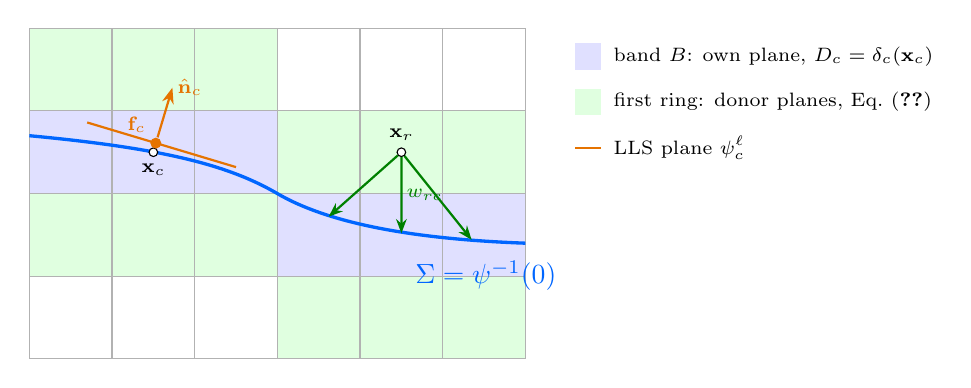
\begin{tikzpicture}[scale=1.05]
    % mesh
    \foreach \i in {0,...,6} { \draw[meshline] (\i,0) -- (\i,4); }
    \foreach \j in {0,...,4} { \draw[meshline] (0,\j) -- (6,\j); }
    % band cells (interface crosses them) and ring cells
    \foreach \p in {(0,2),(1,2),(2,2),(3,1),(4,1),(5,1)}
      { \fill[bandcell] \p rectangle +(1,1); }
    \foreach \p in {(0,1),(1,1),(2,1),(3,0),(4,0),(5,0),
                    (0,3),(1,3),(2,3),(3,2),(4,2),(5,2)}
      { \fill[ringcell] \p rectangle +(1,1); }
    % redraw mesh over fills
    \foreach \i in {0,...,6} { \draw[meshline] (\i,0) -- (\i,4); }
    \foreach \j in {0,...,4} { \draw[meshline] (0,\j) -- (6,\j); }
    % interface: gentle curve through the band cells (crosses rows at x = 3)
    \draw[interface]
      (0,2.7) .. controls (1.6,2.55) and (2.4,2.35) .. (3,2.0)
              .. controls (3.6,1.65) and (4.6,1.45) .. (6,1.4);
    \node[blue!60!cyan, anchor=north west] at (4.55,1.3)
      {$\Sigma=\psilev^{-1}(0)$};
    % LLS plane in band cell (1,2)-(2,3): centre at (1.5,2.5)
    \draw[planeline] (0.7,2.86) -- (2.5,2.32);
    \node[cellcentre, label={[label distance=-1pt]below:{\scriptsize $\xc$}}]
      (xc) at (1.5,2.5) {};
    \node[foot,
      label={[label distance=-2pt, orange!90!black]above left:{\scriptsize $\mathbf{f}_c$}}]
      (fc) at (1.53,2.61) {};
    \draw[normalvec] (fc) -- +(0.20,0.67)
      node[anchor=west, inner sep=1.5pt] {\scriptsize $\nhat_c$};
    % ring cell donor arrows: ring cell centre (4.5, 2.5)
    \node[cellcentre, label={[label distance=-1pt]above:{\scriptsize $\mathbf{x}_r$}}]
      (xr) at (4.5,2.5) {};
    \draw[donorarrow] (xr) -- (3.62,1.72);
    \draw[donorarrow] (xr) -- (4.5,1.52)
      node[midway, anchor=west, inner sep=1.5pt,
           green!50!black] {\scriptsize $w_{rc}$};
    \draw[donorarrow] (xr) -- (5.35,1.44);
    % legend
    \fill[bandcell] (6.6,3.5) rectangle +(0.32,0.32);
    \node[anchor=west] at (6.95,3.66) {\scriptsize band $B$: own plane, $D_c=\delta_c(\xc)$};
    \fill[ringcell] (6.6,2.95) rectangle +(0.32,0.32);
    \node[anchor=west] at (6.95,3.11) {\scriptsize first ring: donor planes, Eq.~(\ref{eq:ring})};
    \draw[planeline] (6.6,2.55) -- (6.92,2.55);
    \node[anchor=west] at (6.95,2.55) {\scriptsize LLS plane $\psilev^{\ell}_c$};
  \end{tikzpicture}
  \caption{Plane anchors. Band cells (blue) fit the least-squares plane
    (\ref{eq:lls}) and anchor their own signed plane distance; the plane foot
    $\mathbf{f}_c$ and unit normal $\nhat_c$ become the wave seed. First-ring
    cells (green) anchor the plicRDF-weighted evaluation of the adjacent
    donor planes.}
  \label{fig:anchors}
\end{figure}

\subsection{The donor-plane wave fill}
\label{sec:wave}
The remaining field is filled by a nearest-donor propagation built on
OpenFOAM's parallel-native \textsc{MeshWave}/\textsc{FaceCellWave}. Every
face of every band anchor cell is seeded with the cell's donor plane
$(\mathbf{f}_c, \nhat_c)$ and the ordering metric
$|\mathbf{x}_f-\mathbf{f}_c|^2$ (a face shared by two anchors keeps the
closer donor). The wave transports, per cell, the donor with the minimal
foot-point distance --- the propagation is monotone and causal, and
terminates in $\mathcal{O}(N)$ operations without linear solves. The
\emph{received value}, however, is not the discrete foot-point distance but
the \emph{continuous} evaluation of the donor plane,
\begin{equation}
  \psilev_{new}(\xc)
  = \operatorname{sign}(\psilev_{old,c})\,
    \big|(\xc-\mathbf{f})\cdot\nhat\big|,
  \label{eq:wave}
\end{equation}
followed by the exact anchor override on band and ring. Cells never reached
by the wave (an interface that left the domain or a disconnected region)
keep $|\psilev_{old}|$ with their old sign.

The distinction in (\ref{eq:wave}) is the load-bearing design decision
(Figure~\ref{fig:donorplane}). The min-over-feet distance field
$\min_i|\mathbf{x}-\mathbf{f}_i|$ is a union of cones: its level sets bulge
between the discrete feet (sagitta $\approx s^2/8d$ at foot spacing $s$),
and its gradient kinks at every donor boundary. Those kinks land exactly on
the band norm $\,||\gradpsi|-1|\,$ that the trigger criterion polices ---
measured on the static gate, the point-cloud variant \emph{raised} the band
deviation an event must lower (Section~\ref{sec:negative}). Evaluating the
donor plane removes the scalloping structurally: moving parallel to the
plane does not change the value, and for a \emph{planar} interface every
donor evaluates the same plane, so the redistanced field is globally exact
to machine precision. For curved interfaces the donor plane is the
least-squares tangent plane at the nearest anchor, and the evaluation error
grows as $\mathcal{O}(|\mathbf{x}-\mathbf{f}|^2\kappa)$ --- second order at
the band scale that feeds the phase indicator and the trigger criterion.

\begin{figure}[htbp]
  \centering
  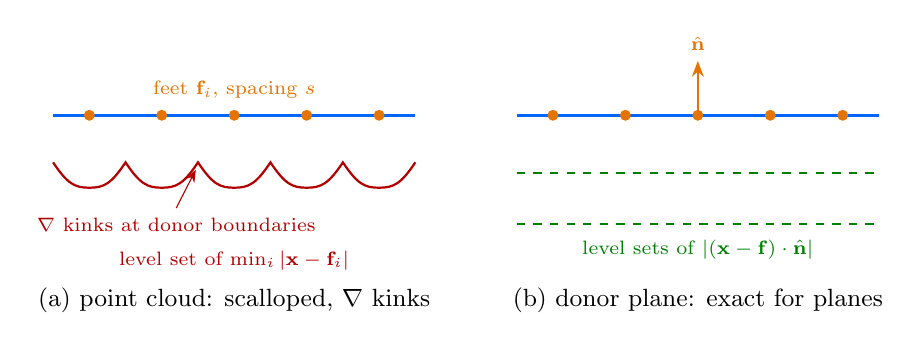
\begin{tikzpicture}[scale=0.92]
    % ---------------- left: point-cloud distance (v1, rejected) ------------
    \begin{scope}
      \draw[interface] (0,3) -- (5,3);
      \foreach \x in {0.5,1.5,2.5,3.5,4.5} { \node[foot] at (\x,3) {}; }
      \node[orange!90!black] at (2.5,3.35) {\scriptsize feet $\mathbf{f}_i$, spacing $s$};
      % scalloped level set: circular bulges under each foot, kinks midway
      \draw[scallop]
        (0,2.35) .. controls (0.2,2.05) and (0.3,2.0) .. (0.5,2.0)
                 .. controls (0.7,2.0) and (0.8,2.05) .. (1,2.35)
                 .. controls (1.2,2.05) and (1.3,2.0) .. (1.5,2.0)
                 .. controls (1.7,2.0) and (1.8,2.05) .. (2,2.35)
                 .. controls (2.2,2.05) and (2.3,2.0) .. (2.5,2.0)
                 .. controls (2.7,2.0) and (2.8,2.05) .. (3,2.35)
                 .. controls (3.2,2.05) and (3.3,2.0) .. (3.5,2.0)
                 .. controls (3.7,2.0) and (3.8,2.05) .. (4,2.35)
                 .. controls (4.2,2.05) and (4.3,2.0) .. (4.5,2.0)
                 .. controls (4.7,2.0) and (4.8,2.05) .. (5,2.35);
      \draw[-{Stealth[length=1.6mm]}, red!70!black, thin]
        (1.7,1.72) -- (1.97,2.25);
      \node[red!70!black, anchor=north] at (1.7,1.72)
        {\scriptsize $\nabla$ kinks at donor boundaries};
      \node[red!70!black] at (2.5,1.0)
        {\scriptsize level set of $\min_i|\mathbf{x}-\mathbf{f}_i|$};
      \node at (2.5,0.45) {\small (a) point cloud: scalloped, $\nabla$ kinks};
    \end{scope}
    % ---------------- right: donor-plane evaluation (final) ----------------
    \begin{scope}[xshift=6.4cm]
      \draw[interface] (0,3) -- (5,3);
      \foreach \x in {0.5,1.5,2.5,3.5,4.5} { \node[foot] at (\x,3) {}; }
      \draw[normalvec] (2.5,3) -- (2.5,3.75)
        node[anchor=south] {\scriptsize $\nhat$};
      % flat level lines
      \foreach \y in {2.2,1.5} { \draw[levelline] (0,\y) -- (5,\y); }
      \node[green!50!black] at (2.5,1.15)
        {\scriptsize level sets of $|(\mathbf{x}-\mathbf{f})\cdot\nhat|$};
      \node at (2.5,0.45) {\small (b) donor plane: exact for planes};
    \end{scope}
  \end{tikzpicture}
  \caption{The wave's received value. (a) Distance to the discrete foot-point
    cloud: level sets scallop between feet and the gradient kinks at donor
    boundaries --- the measured resolution-independent floor on the band
    deviation. (b) Continuous evaluation of the donor plane
    (\ref{eq:wave}): scalloping removed structurally; machine-exact for
    planar interfaces.}
  \label{fig:donorplane}
\end{figure}

\subsection{Algorithm and properties}
\label{sec:algorithm}
One redistance event of \texttt{planeFootWave} executes:
\begin{enumerate}
  \item build the anchor set (Section~\ref{sec:anchors}): one pass over the
    band with a single matched halo exchange, one rank-local pass over the
    ring;
  \item seed all faces of the band cells with $(\mathbf{f}_c,\nhat_c,
    |\mathbf{x}_f-\mathbf{f}_c|^2)$, deduplicated per face by the smaller
    metric;
  \item propagate with \textsc{FaceCellWave} (processor, cyclic and AMI
    boundaries handled natively);
  \item evaluate (\ref{eq:wave}) in every reached cell, re-sign from
    $\psilev_{old}$, keep $|\psilev_{old}|$ in unreached cells;
  \item override band and ring cells with their exact anchor distances.
\end{enumerate}
The model is parameter-free and solver-free; its cost is dominated by the
$\mathcal{O}(N)$ wave with a small constant. Signs never change outside the
band, so redistancing cannot alter topology in the bulk; inside the band the
exact plane distances may legitimately realign a cut-cell centre by a
sub-cell amount, which is why the calling solver refreshes the narrow band
and the phase indicator after every event and logs the interface-volume
shift. Consistency with the phase indicator is structural: both read the
planes of Section~\ref{sec:llsplanes}, so $\alpha$ and the redistanced
$\psilev$ cannot disagree about the interface location.

\subsection{Trigger criterion}
Redistancing fires only when the volume-weighted band mean of
$\,||\gradpsi|-1|\,$ over $\{|\psilev| < 6h\}$ exceeds a threshold
(default $(h/L)^2$), following \cite{abualsaud2018}; every event logs the
interface-volume shift it caused.

% ============================================================================
\section{Software design and reproducibility}
\label{sec:software}
TODO: the \texttt{redistancer} run-time-selection hierarchy
(\texttt{noRedistancing} $|$ \texttt{PDE} $|$ \texttt{planeFootWave} $|$
\texttt{anchoredEikonal}), the shared plane-reconstruction code path with the
phase indicator, and the snakemake test-suite. All results reproduce with
\texttt{make studies-grl}.

% ============================================================================
\section{Verification}
\label{sec:verification}

\subsection{Static redistancing gate}
\label{sec:static}
A circle ($R=0.25$) in the unit square is initialized as the saturating
profile $\psilev_0 = \ell\tanh(d/(\ell\varepsilon))$, $\ell=0.1$,
$\varepsilon=0.5$: the zero set is exact while
$|\gradpsi|(\Sigma) = 2$. One redistance event is applied and measured
against the analytic signed distance over the band
$\{|\psilev_{exact}|\le 6h\}$. Table~\ref{tab:static} and
Figure~\ref{fig:static} show second-order convergence of the plane-anchored
models, with the donor-plane wave roughly an order of magnitude more
accurate than the anchored-Eikonal fill; PDE reinitialization
\cite{sussman1994} \emph{increases} the band error at every resolution
(see Section~\ref{sec:negative}).

\begin{table}[htbp]
  \centering
  \caption{Static gate: band $L_\infty(\psilev-\psilev_{exact})$ before and
           after one redistance event, and observed convergence orders.}
  \label{tab:static}
  \begin{tabular}{l r r r r}
\hline
redistancer & $h$ & pre-event & post-event & order \\
\hline
PDE & 0.0039062 & 2.03e-02 & 4.07e-02 & -- \\
PDE & 0.0078125 & 2.66e-02 & 8.90e-02 & 1.13 \\
PDE & 0.015625 & 2.66e-02 & 1.74e-01 & 0.97 \\
PDE & 0.03125 & 8.59e-02 & 3.67e-01 & 1.07 \\
\hline
anchoredEikonal & 0.0039062 & 2.03e-02 & 3.53e-04 & -- \\
anchoredEikonal & 0.0078125 & 2.66e-02 & 1.40e-03 & 1.98 \\
anchoredEikonal & 0.015625 & 2.66e-02 & 5.80e-03 & 2.06 \\
anchoredEikonal & 0.03125 & 8.59e-02 & 2.97e-02 & 2.35 \\
\hline
planeFootWave & 0.0039062 & 2.03e-02 & 4.48e-05 & -- \\
planeFootWave & 0.0078125 & 2.66e-02 & 1.76e-04 & 1.97 \\
planeFootWave & 0.015625 & 2.66e-02 & 7.02e-04 & 2.00 \\
planeFootWave & 0.03125 & 8.59e-02 & 4.08e-03 & 2.54 \\
\hline
\end{tabular}

\end{table}

\begin{figure}[htbp]
  \centering
  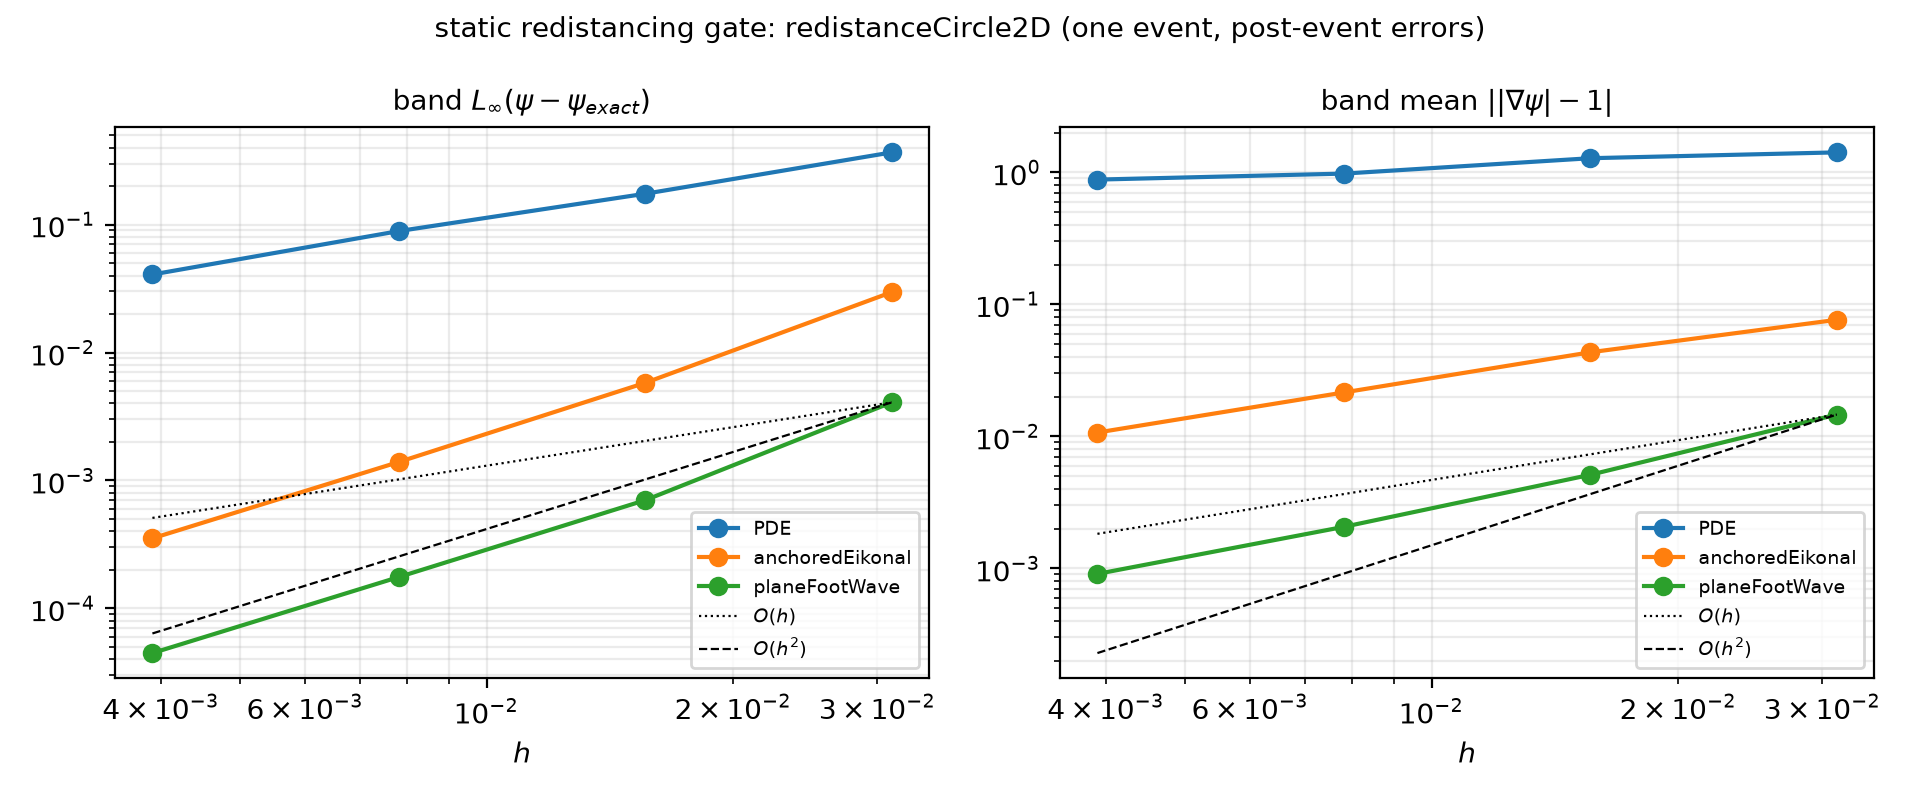
\includegraphics[width=0.95\linewidth]{static_redistance_convergence.png}
  \caption{Static gate convergence: post-event band error norms per
           redistancer model, with $O(h)$ and $O(h^2)$ guides.}
  \label{fig:static}
\end{figure}

\subsection{Interface displacement by a single redistancing step}
\label{sec:idempotency}
Redistancing an \emph{exact} signed distance function must leave the
interface position, the phase volume and the signed-distance profile
unchanged: any measured deviation is the interface displacement and
spurious volume change that ONE redistancing step introduces --- the
classical concern about reinitialization \cite{sussman1994,russo2000},
and exactly the error that accumulates when redistancing is applied
repeatedly during advection. The test initializes $\psilev$ as the exact
signed distance of (a) a circle ($R=0.15$, centred in the unit square, the
reversed-vortex interface) and (b) the diagonal plane through the centre,
applies one redistancing step, and compares with the input over
$N \in \{32,\dots,256\}$ (Table~\ref{tab:idempotency},
Figure~\ref{fig:idemFieldsCircle}). Measured: \texttt{noRedistancing}
(control) changes nothing; \texttt{planeFootWave} preserves a planar
interface to machine precision ($10^{-14}$, volume change
$\sim\!10^{-16}$) and is second order on the circle --- the spurious
volume change per redistancing step converges as $\mathcal{O}(h^2)$
($1.05\!\cdot\!10^{-4} \to 1.72\!\cdot\!10^{-6}$, ratio $\approx 4$ per
level; $1.5\%$ of the phase volume at $N=32$, $0.02\%$ at $N=256$).
$E_{geom} = E_{vol}$ \emph{exactly} at every resolution: the interface
displacement is one-signed --- the least-squares chord-plane bias of
Section~\ref{sec:anchors}, not noise. \texttt{anchoredEikonal} shows the
identical volume change (the interface position is set by the shared
anchors, not by the far-field distance propagation) but first-order band
$\psilev$ error on the plane; the PDE baseline displaces the interface
strongly at coarse $N$ ($0.2$ band error at $N=32$).

\begin{table}[htbp]
  \centering
  \caption{Interface displacement and volume conservation of a single
    redistancing step applied to an exact signed distance.}
  \label{tab:idempotency}
  \resizebox{\linewidth}{!}{\begin{tabular}{l l r r r r r}
\hline
surface & redistancer & $h$ & band $L_\infty(\psi)$ & order & $E_{vol}$ & $E_{geom}$ \\
\hline
circle & PDE & 0.0039062 & 1.06e-05 & -- & 7.45e-09 & 2.13e-08 \\
circle & PDE & 0.0078125 & 4.59e-04 & 5.43 & 4.23e-08 & 1.51e-07 \\
circle & PDE & 0.015625 & 4.34e-02 & 6.56 & 1.79e-04 & 1.09e-03 \\
circle & PDE & 0.03125 & 1.97e-01 & 2.18 & 6.63e-03 & 6.63e-03 \\
\hline
circle & anchoredEikonal & 0.0039062 & 5.64e-04 & -- & 1.17e-07 & 1.20e-07 \\
circle & anchoredEikonal & 0.0078125 & 2.28e-03 & 2.01 & 4.59e-07 & 4.78e-07 \\
circle & anchoredEikonal & 0.015625 & 9.74e-03 & 2.10 & 1.59e-06 & 1.59e-06 \\
circle & anchoredEikonal & 0.03125 & 2.93e-02 & 1.59 & 1.11e-05 & 1.11e-05 \\
\hline
circle & noRedistancing & 0.0039062 & 5.00e-14 & -- & 0.00e+00 & 0.00e+00 \\
circle & noRedistancing & 0.0078125 & 4.99e-14 & -0.00 & 0.00e+00 & 0.00e+00 \\
circle & noRedistancing & 0.015625 & 4.99e-14 & -0.00 & 0.00e+00 & 0.00e+00 \\
circle & noRedistancing & 0.03125 & 4.48e-13 & 3.16 & 0.00e+00 & 0.00e+00 \\
\hline
circle & planeFootWave & 0.0039062 & 9.47e-05 & -- & 1.17e-07 & 1.20e-07 \\
circle & planeFootWave & 0.0078125 & 3.79e-04 & 2.00 & 4.59e-07 & 4.78e-07 \\
circle & planeFootWave & 0.015625 & 1.44e-03 & 1.93 & 1.59e-06 & 1.59e-06 \\
circle & planeFootWave & 0.03125 & 4.88e-03 & 1.76 & 1.11e-05 & 1.11e-05 \\
\hline
plane & PDE & 0.0039062 & 1.00e-11 & -- & 4.22e-15 & 3.45e-14 \\
plane & PDE & 0.0078125 & 9.33e-12 & -0.10 & 5.83e-14 & 6.20e-14 \\
plane & PDE & 0.015625 & 2.93e-11 & 1.65 & 9.39e-14 & 2.07e-13 \\
plane & PDE & 0.03125 & 8.53e-11 & 1.54 & 8.96e-13 & 1.42e-12 \\
\hline
plane & anchoredEikonal & 0.0039062 & 1.84e-03 & -- & 2.36e-16 & 1.09e-15 \\
plane & anchoredEikonal & 0.0078125 & 3.68e-03 & 1.00 & 4.16e-16 & 9.15e-16 \\
plane & anchoredEikonal & 0.015625 & 7.43e-03 & 1.01 & 5.97e-16 & 1.07e-15 \\
plane & anchoredEikonal & 0.03125 & 1.49e-02 & 1.00 & 1.04e-16 & 1.56e-16 \\
\hline
plane & noRedistancing & 0.0039062 & 5.00e-14 & -- & 0.00e+00 & 0.00e+00 \\
plane & noRedistancing & 0.0078125 & 4.10e-14 & -0.28 & 0.00e+00 & 0.00e+00 \\
plane & noRedistancing & 0.015625 & 4.09e-14 & -0.00 & 0.00e+00 & 0.00e+00 \\
plane & noRedistancing & 0.03125 & 4.78e-13 & 3.55 & 0.00e+00 & 0.00e+00 \\
\hline
plane & planeFootWave & 0.0039062 & 1.61e-13 & -- & 2.36e-16 & 1.09e-15 \\
plane & planeFootWave & 0.0078125 & 1.60e-13 & -0.01 & 4.16e-16 & 9.15e-16 \\
plane & planeFootWave & 0.015625 & 7.75e-14 & -1.04 & 5.97e-16 & 1.07e-15 \\
plane & planeFootWave & 0.03125 & 1.33e-14 & -2.55 & 1.04e-16 & 1.56e-16 \\
\hline
\end{tabular}
}
\end{table}

\begin{figure}[htbp]
  \centering
  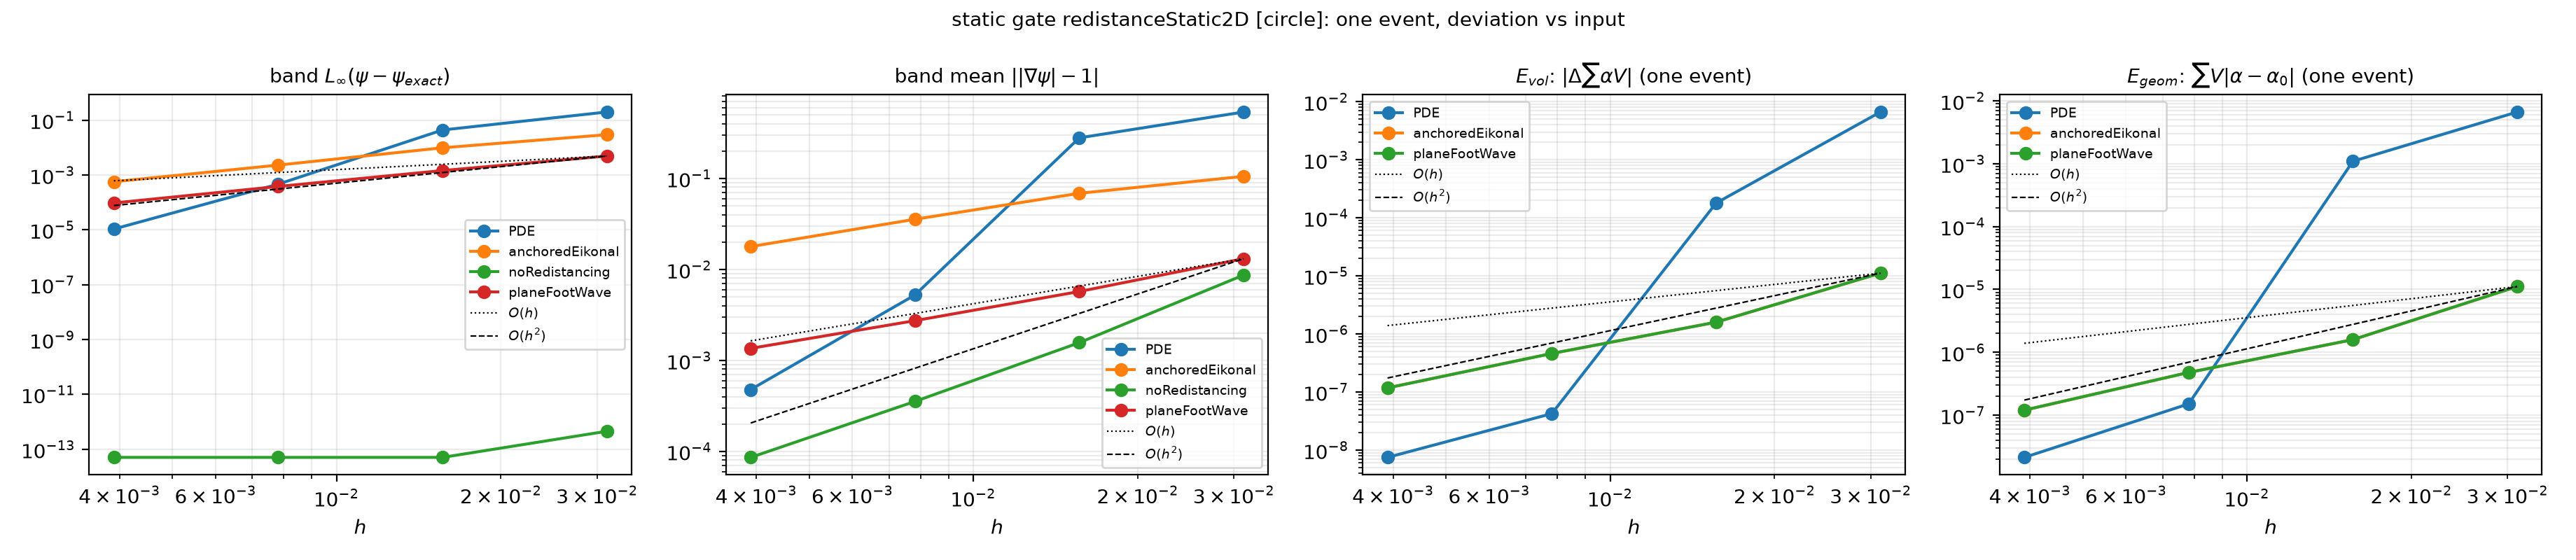
\includegraphics[width=0.95\linewidth]{redistanceStatic2D_convergence_circle.png}\\
  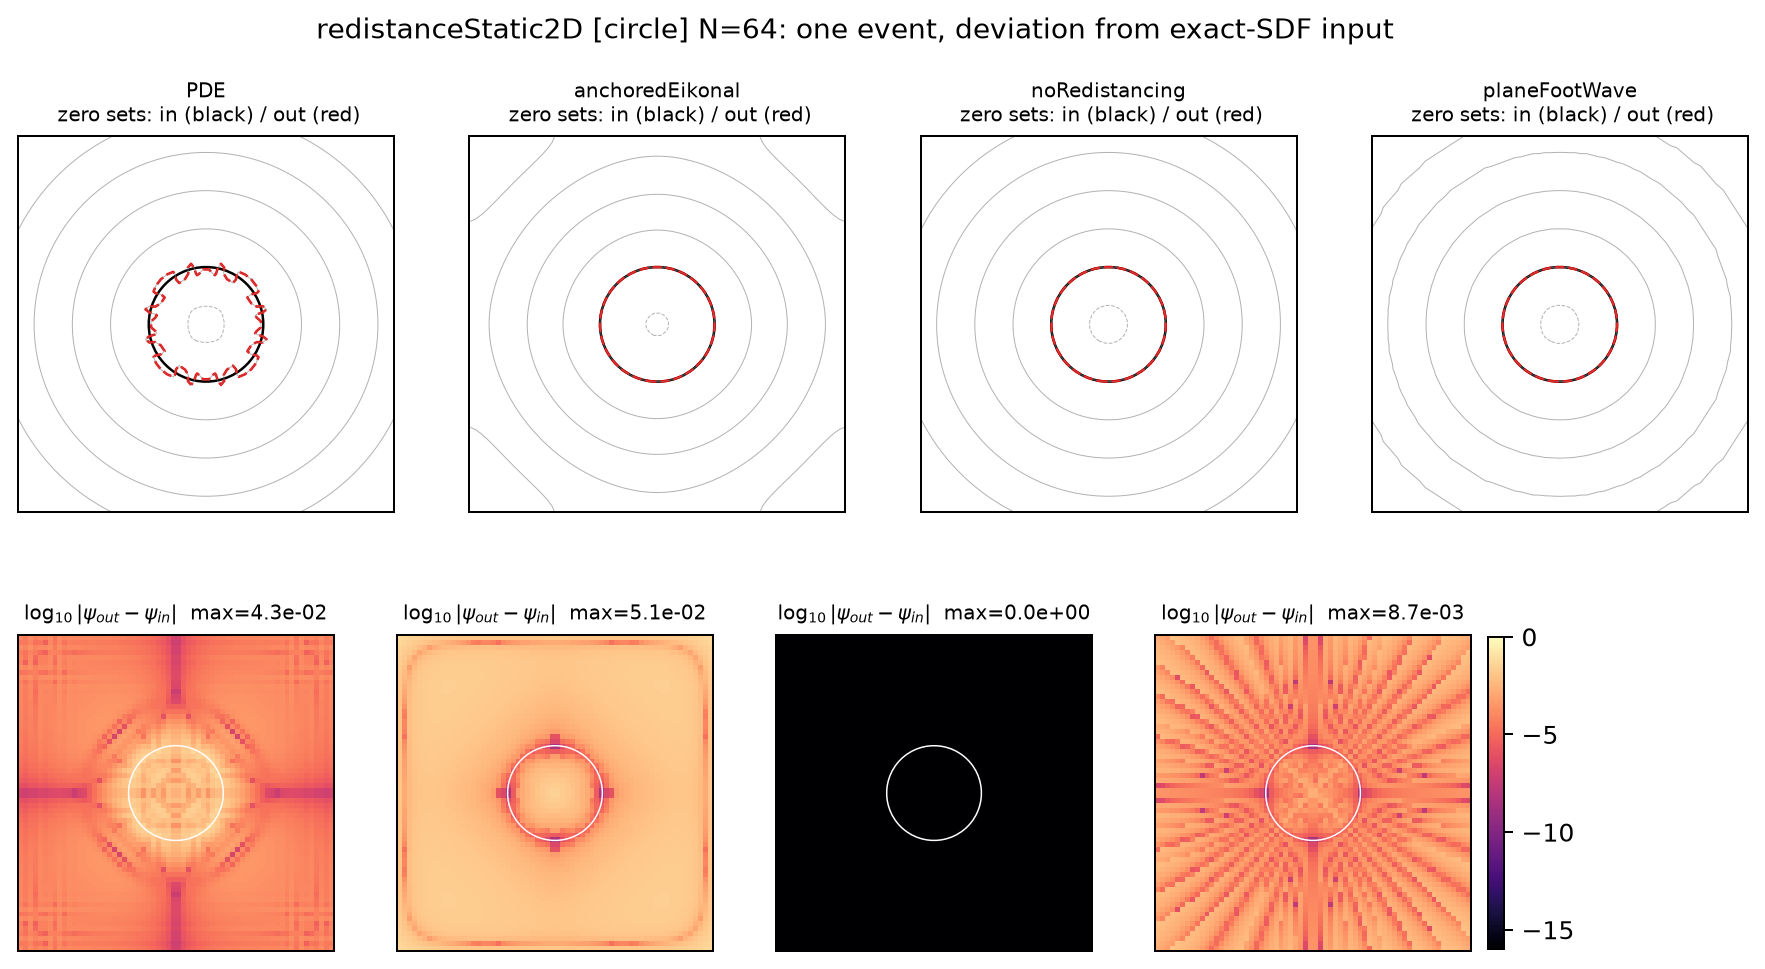
\includegraphics[width=0.95\linewidth]{redistanceStatic2D_fields_circle.png}
  \caption{Redistancing an exact signed distance of a circle: convergence
    of the interface displacement, volume and shape errors (top) and
    per-model field plots (bottom; input/output zero level sets and
    $\log_{10}|\psilev_{out}-\psilev_{in}|$). Plane-interface counterparts:
    \texttt{redistanceStatic2D\_\{convergence,fields\}\_plane.png}.}
  \label{fig:idemFieldsCircle}
\end{figure}

\subsection{Reversed vortex (2D)}
TODO: \texttt{bulkVortexGRL} — shape/volume/band-gradient errors and event
counts vs.\ \texttt{noRedistancing} and the PDE baseline.
% \begin{tabular}{l l l r r r}
\hline
study & redistancer & cfl & $h$ & shape error & order \\
\hline
bulkVortexGRL & PDE & 0.5 & 0.03125 & 4.97e-02 & -- \\
bulkVortexGRL & PDE & 0.5 & 0.015625 & 1.02e-02 & 2.29 \\
bulkVortexGRL & PDE & 0.5 & 0.0078125 & 4.43e-03 & 1.20 \\
\hline
bulkVortexGRL & PDE & 1.0 & 0.03125 & 4.99e-02 & -- \\
bulkVortexGRL & PDE & 1.0 & 0.015625 & 1.02e-02 & 2.29 \\
bulkVortexGRL & PDE & 1.0 & 0.0078125 & 4.44e-03 & 1.20 \\
\hline
bulkVortexGRL & anchoredEikonal & 0.5 & 0.03125 & 4.97e-02 & -- \\
bulkVortexGRL & anchoredEikonal & 0.5 & 0.015625 & 5.06e-02 & -0.02 \\
bulkVortexGRL & anchoredEikonal & 0.5 & 0.0078125 & 5.00e-02 & 0.02 \\
\hline
bulkVortexGRL & anchoredEikonal & 1.0 & 0.03125 & 4.96e-02 & -- \\
bulkVortexGRL & anchoredEikonal & 1.0 & 0.015625 & 5.09e-02 & -0.04 \\
bulkVortexGRL & anchoredEikonal & 1.0 & 0.0078125 & 5.02e-02 & 0.02 \\
\hline
bulkVortexGRL & noRedistancing & 0.5 & 0.03125 & 6.97e-03 & -- \\
bulkVortexGRL & noRedistancing & 0.5 & 0.015625 & 7.04e-03 & -0.02 \\
bulkVortexGRL & noRedistancing & 0.5 & 0.0078125 & 2.20e-03 & 1.68 \\
\hline
bulkVortexGRL & noRedistancing & 1.0 & 0.03125 & 6.97e-03 & -- \\
bulkVortexGRL & noRedistancing & 1.0 & 0.015625 & 7.04e-03 & -0.02 \\
bulkVortexGRL & noRedistancing & 1.0 & 0.0078125 & 2.20e-03 & 1.68 \\
\hline
bulkVortexGRL & planeFootWave & 0.5 & 0.03125 & 3.59e-02 & -- \\
bulkVortexGRL & planeFootWave & 0.5 & 0.015625 & 4.90e-02 & -0.45 \\
bulkVortexGRL & planeFootWave & 0.5 & 0.0078125 & 5.09e-02 & -0.06 \\
\hline
bulkVortexGRL & planeFootWave & 1.0 & 0.03125 & 6.32e-02 & -- \\
bulkVortexGRL & planeFootWave & 1.0 & 0.015625 & 4.97e-02 & 0.35 \\
bulkVortexGRL & planeFootWave & 1.0 & 0.0078125 & 4.82e-02 & 0.05 \\
\hline
\end{tabular}

% 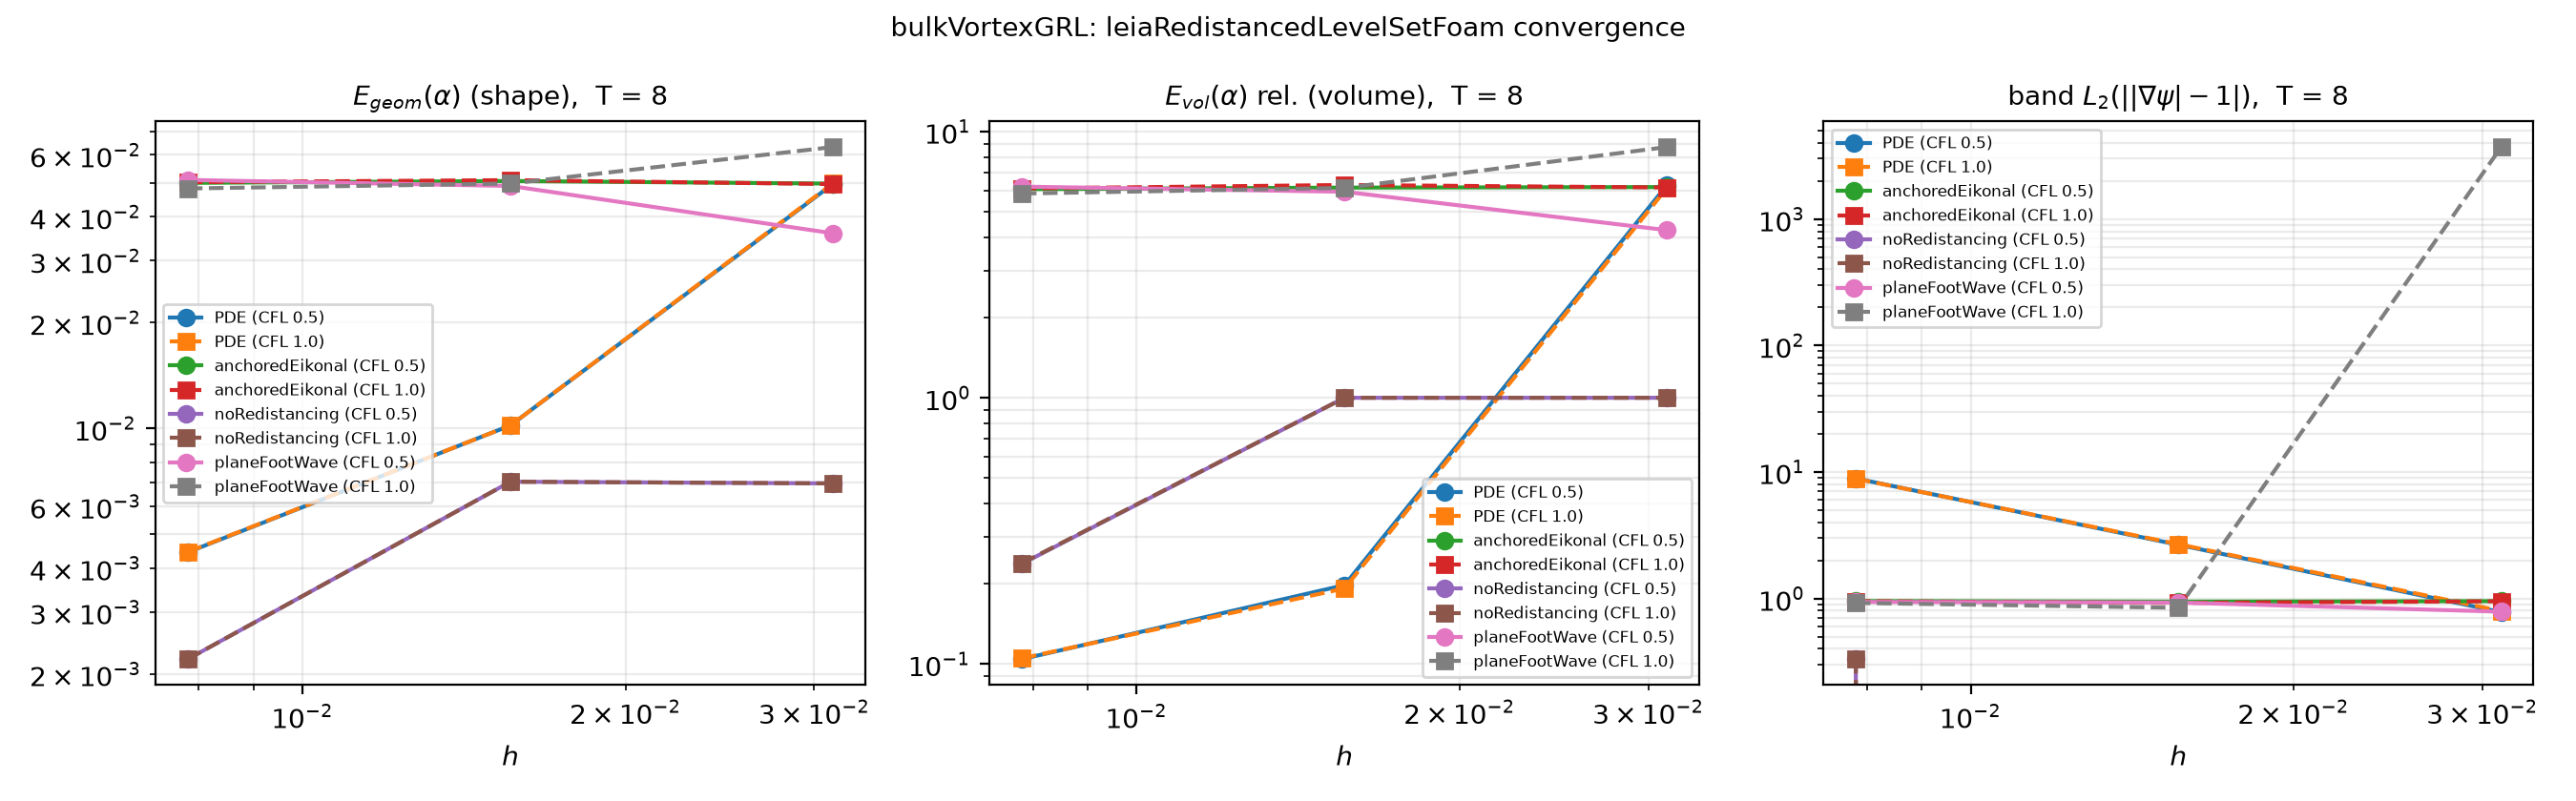
\includegraphics[width=\linewidth]{bulkVortexGRL_convergence.png}

\subsection{Three-dimensional shear and deformation}
TODO: \texttt{3DshearGRL}, \texttt{3DdeformationGRL} (hex), iso-surface
montages.

\subsection{Trigger ablation}
TODO: \texttt{vortexTriggerGRL} — every-step (interval) vs.\ criterion-gated
redistancing.

% ============================================================================
\section{Negative results}
\label{sec:negative}
Measured dead ends and their mechanisms are first-class results of this
line; the companion deck (\texttt{grl-negative-results}) documents each with
the pass criterion \emph{a redistance event must not injure the field}:
\begin{enumerate}
  \item \textbf{Foot-point-cloud distances scallop the gradient}: the
    min-over-feet distance field has scalloped level sets whose kinks land
    exactly on the band norm the trigger polices; replaced by the continuous
    donor-plane evaluation (\ref{eq:wave}).
  \item \textbf{The anchored-Eikonal fill is first order in the band}: with
    a sufficient iteration budget it converges, yet its upwind
    advection-diffusion linearization \cite{tucker2003} leaves an
    $\mathcal{O}(h)$ error inside the trigger band on exact planar fields;
    it is retained as the documented comparison model.
  \item \textbf{PDE reinitialization}: a fixed pseudo-time step is a
    mesh-dependent stability bomb, and even a CFL-safe step injures
    saturated profiles through the non-Godunov central Hamiltonian
    discretization; cures exist \cite{russo2000} but the geometric route
    sidesteps them.
\end{enumerate}

% ============================================================================
\section{Limitations and outlook}
\label{sec:outlook}
TODO: filaments below the $\sim 2h$ plane-fit resolution limit; polyhedral
and perturbed meshes; two-phase coupling.

% ============================================================================
\section{Conclusions}
\label{sec:conclusions}
TODO.

\bibliographystyle{elsarticle-num}
\bibliography{refs}

\end{document}
